\documentclass[t,compress]{beamer}
%\documentclass[t,compress,handout]{beamer}

\newcommand{\by}{\boldsymbol{y}}
\newcommand{\btheta}{\boldsymbol{\theta}}
\newcommand{\bd}{\boldsymbol{d}}
\newcommand{\bx}{\boldsymbol{x}}
\newcommand{\br}{\boldsymbol{r}}

\usepackage{amsmath,amsfonts,amssymb}
\usepackage[normalem]{ulem} 
\usepackage{booktabs} 
\usepackage[english]{babel}

\usetheme{Madrid}
\pagestyle{empty}
%
\setcounter{section}{0}

%\RequirePackage[osf,sc]{mathpazo}{}
\RequirePackage[scaled=0.90]{helvet}{}
\RequirePackage[scaled=0.85]{beramono}{}
\RequirePackage[T1]{fontenc}
\RequirePackage{textcomp}
\graphicspath{{graphics/}}
%%%%%%%%%%%%%%%%%%%%%%%%%%%%%%%%%%%%%%%%%%%%%%%%%%%%%%%%%%%%%%%%%%%%%
%%%%%%%%%%%%%%%%%%%%%%%%%%%%%%%%%%%%%%%%%%%%%%%%%%%%%%%%%%%%%%%%%%%%%
%%%%%%%%%%%%%%%%%%%%%%%%%%%%%%%%%%%%%%%%%%%%%%%%%%%%%%%%%%%%%%%%%%%%%
\title[Bayesian Experimental Design for Stochastic Kinetic Models]{Bayesian
  Experimental Design for Stochastic Kinetic Models}

\author[]{Colin Gillespie, Richard Boys, Nina Wilkinson \\
\bigskip
Newcastle University, UK}

\date{\today}
%%%%%%%%%%%%%%%%%%%%%%%%%%%%%%%%%%%%%%%%%%%%%%%%%%%%%%%%%%%%%%%%%%%%%
%%%%%%%%%%%%%%%%%%%%%%%%%%%%%%%%%%%%%%%%%%%%%%%%%%%%%%%%%%%%%%%%%%%%%
%%%%%%%%%%%%%%%%%%%%%%%%%%%%%%%%%%%%%%%%%%%%%%%%%%%%%%%%%%%%%%%%%%%%%
\begin{document}
\maketitle

\begin{frame}
\frametitle{Overview}
\begin{itemize}
\item Stochastic kinetic models
\item Simulation and inference
\item Optimal design problem
\item Future directions
\end{itemize}

\end{frame}


\begin{frame}
\frametitle{Stochastic kinetic models}

\begin{itemize}
\item A biochemical network is represented as a set of pseudo-biochemical
reactions: for $i=1, \ldots, v$
\[
R_i:~~ p_{i1}\mathcal{X}_1+p_{i2}\mathcal{X}_2+\cdots+p_{iu}\mathcal{X}_u 
~~ \xrightarrow{\theta_i}~~
q_{i1}\mathcal{X}_1+q_{i2}\mathcal{X}_2+\cdots+q_{iu}\mathcal{X}_u
\]
\item Stochastic rate constant $\theta_i$
\item  Hazard/instantaneous rate: $h_i(X_t, \theta_i)$ where $X_t = (X_{1,t}, \ldots, X_{u,t})′$ is
the current state of the system
\item  Under mass-action stochastic kinetics, the hazard function is proportional to a
product of binomial coefficients, with
\[
h_i(X_t,\theta_i) = \theta_i\prod_{j=1}^u \binom{X_{j,t}}{p_{ij}}
\]
\end{itemize}
\end{frame}

\begin{frame}
\frametitle{Stochastic kinetic models}
\begin{itemize}
\item Describe the SKM by a Markov jump process (MJP)
\item The effect of reaction $R_k$ is to change the value of each species $X_i$ by
$q_{ki} - p_{ki}$
\item The time to the next reaction is
\[
t \sim Exp\{h_0 (X_t , \btheta)\}
\]
where $ h_0(X_t, \btheta) =\sum_{i=1}^v h_i(X_i, \theta_i)$
\item The reaction is of type
$i$ with probability $h_i(X_t, \theta_i)/h_0(X_t , \btheta)$
\item The process is easily simulated using the Direct method (Gillespie algorithm)
\end{itemize}
\end{frame}

\begin{frame}

\frametitle{The direct method}

\begin{enumerate}
\item \textbf{Initialisation:} initial conditions, reactions constants, and random number generators
\item \textbf{\alert<2>{Propensities update:}} Update each of the $v$ hazard
  functions, $h_i(X_t, \theta_i)$
\item \textbf{Propensities total:} Calculate the total hazard $h_0 =
  \sum_{i=1}^v h_i(X_t, \theta_i)$
\item \textbf{\alert<3>{Reaction time:}} $\tau = -ln\{U(0,1)\}/h_0$ and $t = t+ \tau$
\item \textbf{\alert<4>{Reaction selection:}} A reaction is chosen proportional to its
  hazard
\item \textbf{Reaction execution:} Update species
\item \textbf{Iteration:} If the simulation time is exceeded stop, otherwise go back to step 2
\end{enumerate}
\alert<2->{Typically a simulated experiment has many simulated reactions}
\end{frame}


\begin{frame}
\frametitle{Parameter estimation: the inverse problem}

\begin{itemize}
\item Given observations on the chemical species, can we infer the rate
  constants, $\theta$?
\item Typically we only partially observe species, at discrete times
\end{itemize}
\begin{figure}[b]
\only<1>{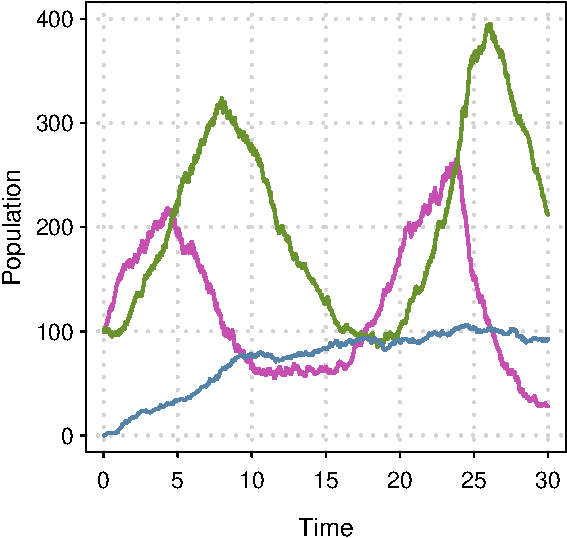
\includegraphics[width=0.45\textwidth]{figure1a-crop.pdf}}%
\only<2>{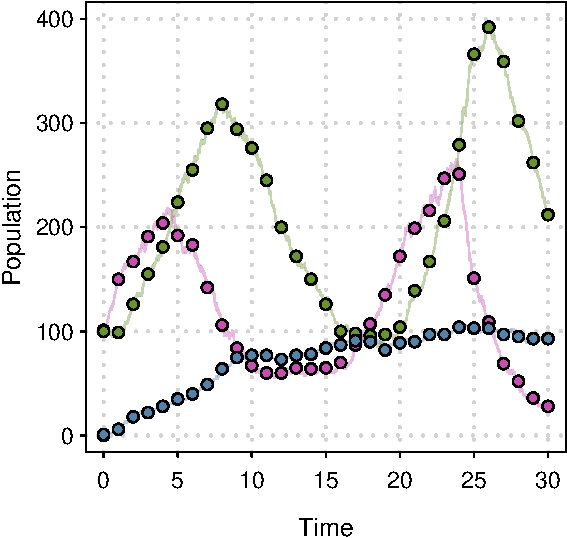
\includegraphics[width=0.45\textwidth]{figure1b-crop.pdf}}%
\only<3>{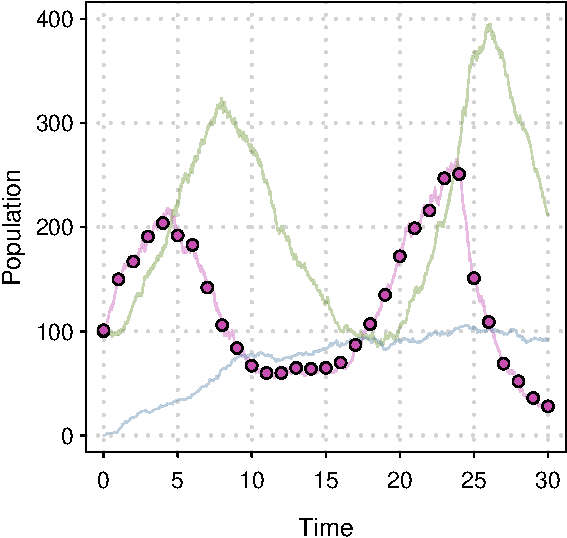
\includegraphics[width=0.45\textwidth]{figure1c-crop.pdf}}%
\only<4>{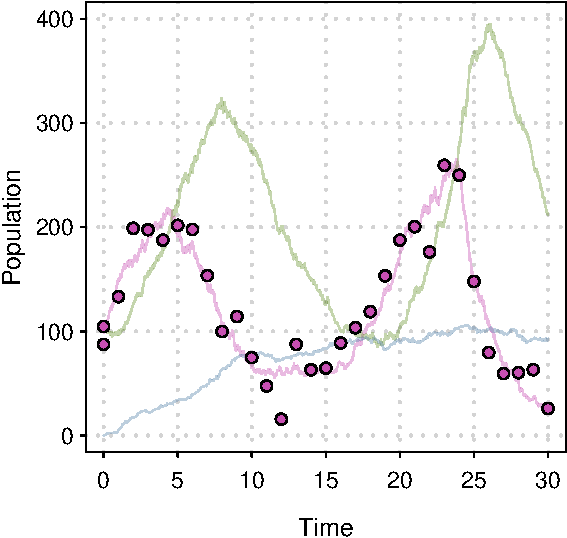
\includegraphics[width=0.45\textwidth]{figure1d-crop.pdf}}%
\end{figure}

\end{frame}

\begin{frame}
\frametitle{Parameter inference}

\begin{block}{Forward simulation approaches}
\begin{itemize}
\item Approximate Bayesian computation (ABC)
\item Particle MCMC
\end{itemize}
\end{block}

\begin{block}{Simulator approximations}
\begin{itemize}
\item Moment closure (2MA)
\item Linear noise approximation (LNA)
\item Langevin equation (SDE)
\item Gaussian processes (GP)
\end{itemize}
\end{block}


\end{frame}

\begin{frame}
\frametitle{Example: The death model}
\begin{columns}[c]
\column{0.63\textwidth}
\begin{itemize}
\item A single reaction
\[
 N \xrightarrow{\theta} \emptyset
\]
\item This model is sufficiently simple that we can obtain the probability of $n$
  individuals at time $t$ analytically
\item Initialising with $N(0) = n_0$ individuals at time $t=0$, we have, for $n=n_0,n_{0}-1,\ldots, 0$
\[
  p_{n}(t)={n_0 \choose n}e^{-\theta n t}(1-e^{-\theta t})^{n_0-n}
\]


\end{itemize}
\column{0.4\textwidth}
\begin{figure}[t]
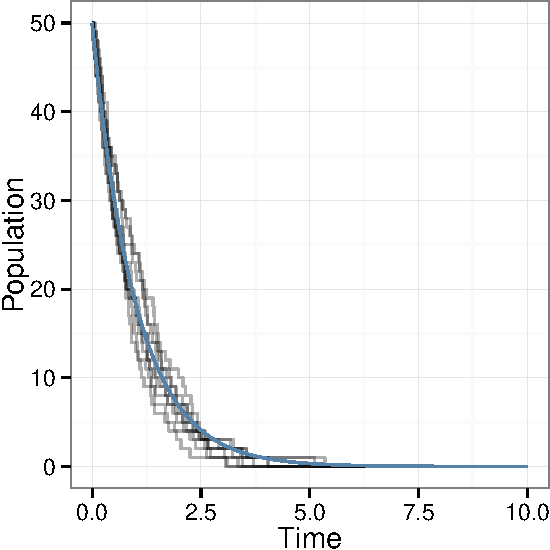
\includegraphics[width=\textwidth]{figure2-crop.pdf} 
\end{figure}
\end{columns}
\end{frame}


\begin{frame}
\frametitle{What would an optimal design look like?}
\begin{block}{}
Suppose we want to observe the process at $k$ time points. What time points
should we use?
\end{block}

\begin{figure}[h]
\only<1>{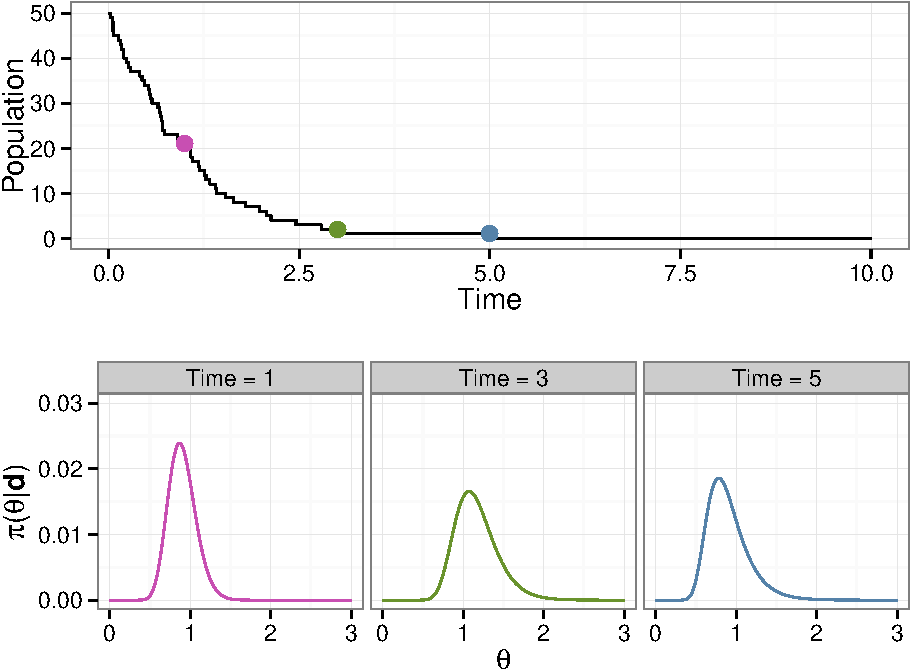
\includegraphics[width=0.6\textwidth]{figure3a-crop.pdf}}%
\only<2>{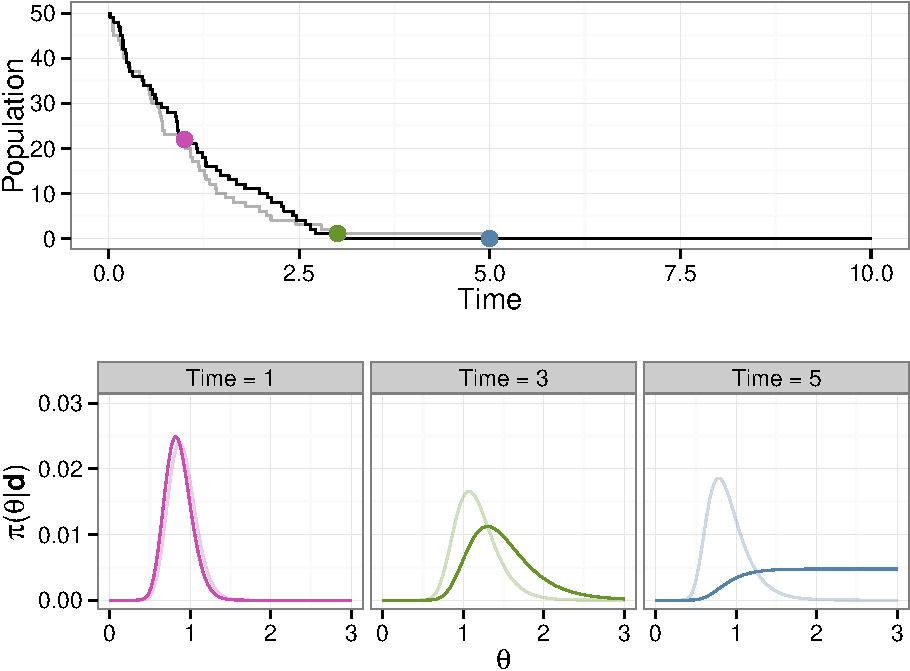
\includegraphics[width=0.6\textwidth]{figure3b-crop.pdf}}%
\only<3>{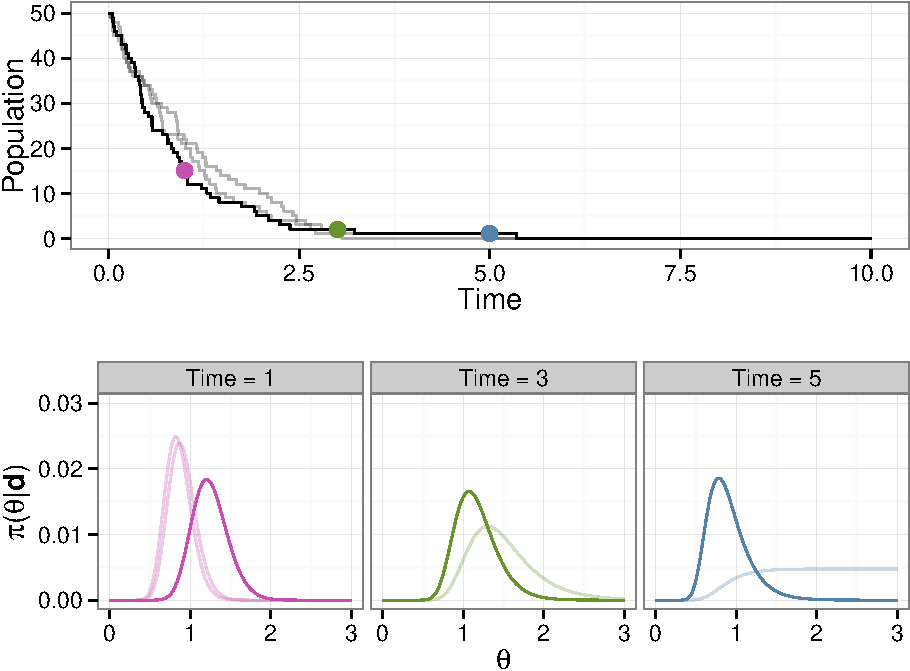
\includegraphics[width=0.6\textwidth]{figure3c-crop.pdf}}%
\end{figure}
\end{frame}

\begin{frame}
\frametitle{Choosing the best design}
\begin{itemize}
\item A typical design is $\bd = (t_1, t_2, \ldots, t_k)$
\item Since the design parameter has to be chosen before doing the experiment we need to maximise 
\[
u(\bd) = E_{\btheta,\by}[u(\bd,\by,\btheta)]=\int_{\by}\int_{\theta}u(\bd,\by,\btheta)\pi(\by|\bd,\btheta)\pi(\btheta)d\btheta d\by
\]
\item The best design $\bd^{\ast}$ maximises $u(\bd)$ 
\item Typically $u(\bd)$ is analytically intractable
\item The utility we choose is
\begin{equation*}
u(\bd,\by,\btheta)\equiv u(\bd,\by)
=\frac{1}{\text{det}\{Var(\btheta | \bd,\by)\}}
\end{equation*}
which does not depend on $\btheta$

\end{itemize} 
\end{frame}



\begin{frame}
\frametitle{Choosing the best design}
\begin{itemize}
\item The utility of a design $\bd = (t_1, t_2, \ldots, t_k)$ is
\begin{align*}
u(\bd)&=E_{\btheta,\by}\left[u(\bd,\by)\right] = \cdots 
%&=\int_{\btheta} \pi(\btheta) \left\{ \int_{\by} u(\bd,\by) \pi(\by | \bd,\btheta) d \by \right\} d \btheta \\
=\int_{\btheta} \pi(\btheta) u(\bd,\btheta) d \btheta \\
\intertext{which can be approximated by}
u(\bd) &= E_{\btheta}\left[u(\bd,\btheta)\right] \simeq \frac{1}{m}\sum_{i=1}^{m} u(\bd,\btheta_i)
\end{align*} 
where the $\btheta_i$ are a random sample of size $m$ from the prior $\pi(\btheta)$
\item Typically, $u(\bd, \btheta)$ is computationally expensive to evaluate
\end{itemize}
\end{frame}


\begin{frame}
\frametitle{Fast approximation $u(\bd, \btheta)$}

\begin{enumerate}
\item Using a Latin hyper-cube design, estimate $u(\bd, \btheta)$ at multiple $(\bd, \btheta)$ points
\item Fit a GP emulator to $u(\bd, \btheta)$, with mean function
\[
m(\bd, \btheta) = \beta_0 + \sum_i \beta_i \theta_i + \sum_j \beta_j d_j 
\]
and a squared exponential covariance function
\[
   K(\bx_i,\bx_j | a, \br ) = a \exp \left \{ (\bx_i-\bx_j)^T
     \text{diag}(\br)^{-2}(\bx_i-\bx_j)\right \}
\]
where  $\bx=(\bd,\btheta)$ 
\item Use the GP emulators within an MCMC scheme to estimate $\bd^*=\text{argmax
  } u(\bd)$

\end{enumerate}

\end{frame}



\begin{frame}
\frametitle{Toy model: Pure death process}
\begin{columns}[c]
\column{0.58\textwidth}
\begin{itemize}
\item Prior: $\theta \sim LN(-0.005, 0.01)$
\item Minimax Latin hypercube design using 400 training points
\item Since we can solve the Master equation, we can calculate the
  utility function exactly
\item For a 1-d design, our approximation is excellent
\item For multiple design points, the approximation is very close to the exact
\item How many design points should we use: what value for $k$?
\end{itemize} 
\column{0.4\textwidth}
\begin{figure}[t]
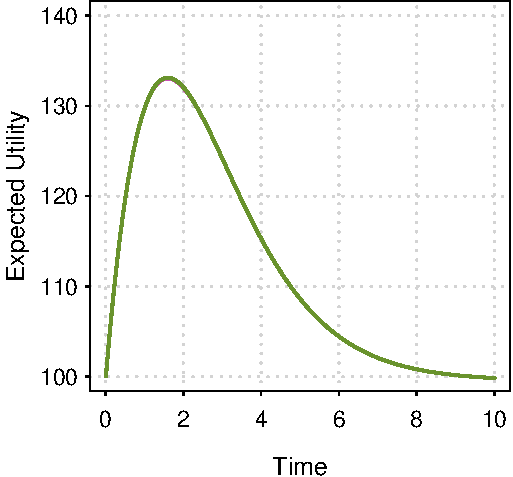
\includegraphics[width=0.8\textwidth]{figure4a-crop.pdf}\\
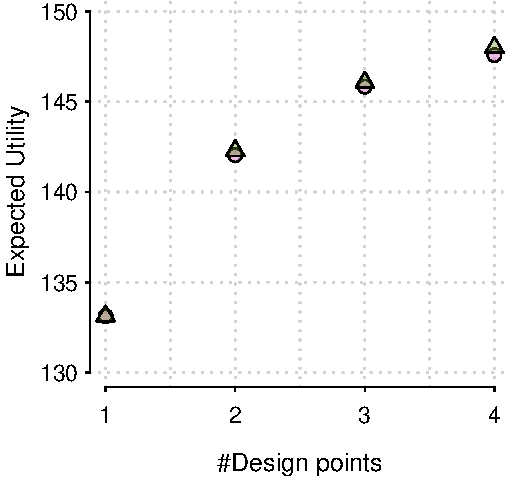
\includegraphics[width=0.8\textwidth]{figure4b-crop.pdf}
\end{figure}
\end{columns}
\end{frame}



\begin{frame}
\frametitle{Results: 2-point design $\bd = (t_1, t_2)$, $t_1 < t_2$}
\begin{figure}[t]
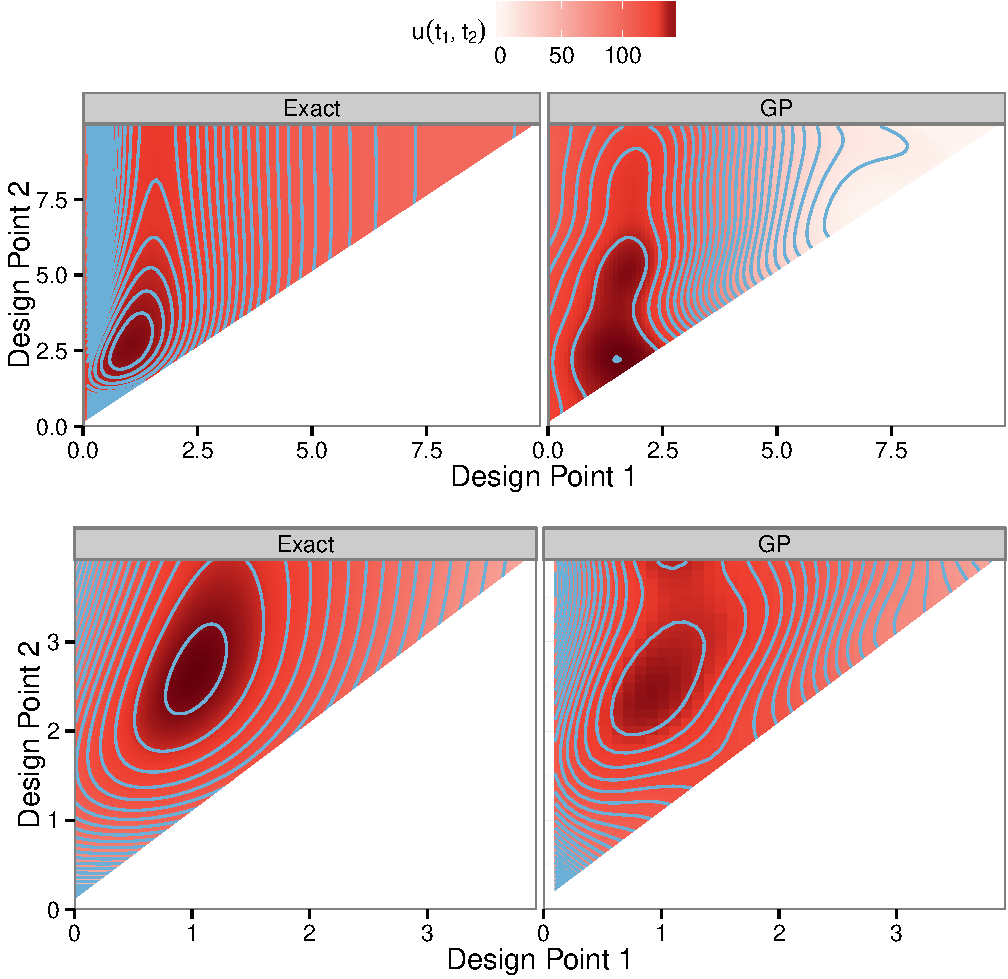
\includegraphics[width=0.65\textwidth]{figure5-crop.pdf}
%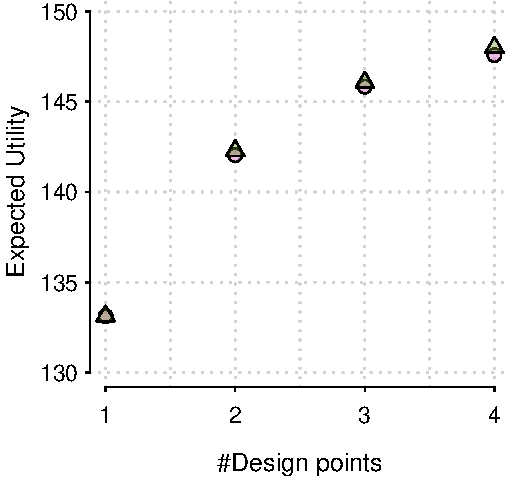
\includegraphics[width=0.8\textwidth]{figure4b-crop.pdf} 
%Legend: u -> u(t_1, t_2)
\end{figure}

\end{frame}

\begin{frame}
\frametitle{Future directions}

\begin{itemize}
\item Current approaches for estimating $u(\bd)$ of SKM do not scale
\item We need to be able to handle larger, more complex models
\item Surface of the utility function is very flat. May need to implement a
  sequential strategy to  gradually zoom into a region around the optimal design $\bd^*$
\item May be useful to use approximations of the stochastic kinetic model to
  focus into the region around the optimal design quickly
\end{itemize}
{\small
Source code (R and \LaTeX\ of these slides):\\
\alert{\url{https://github.com/csgillespie/talks/}}}

\end{frame}











\end{document}

%%% Local Variables: 
%%% mode: latex
%%% TeX-master: t
%%% End: 
